\documentclass[a4paper, 12pt]{article}
\usepackage[T2A,T1]{fontenc}
\usepackage[utf8]{inputenc}
\usepackage[english, russian]{babel}
\usepackage{graphicx}
\usepackage[hcentering, bindingoffset = 10mm, right = 15 mm, left = 15 mm, top=20mm, bottom = 20 mm]{geometry}
\usepackage{multirow}
\usepackage{lipsum}
\usepackage{amsmath, amstext}
\usepackage{siunitx}
\usepackage{wrapfig}
\usepackage{adjustbox}
\usepackage{enumerate, indentfirst, float}
\usepackage{capt-of, svg}
\usepackage{icomma}
\usepackage{fancyhdr}
\usepackage{tabu}
\usepackage{units}

\newenvironment{bottompar}{\par\vspace*{\fill}}{\clearpage}

\pagestyle{fancy}

\rhead{Общая физика МФТИ}
\lhead{Лабораторная работа 2.2.1} 

\renewcommand{\headrulewidth}{2pt}
 
\begin{document}
\begin{titlepage}

\newcommand{\HRule}{\rule{\linewidth}{0.5mm}} % Defines a new command for the horizontal lines, change thickness here


\center % Center everything on the page
 
 
 
%----------------------------------------------------------------------------------------
%	HEADING SECTIONS
%----------------------------------------------------------------------------------------

\textsc{\LARGE Московский Физико-Технический Институт}\\[1,5cm] % Name of your university/college
 % Major heading such as course name
\textsc{\Large Кафедра общей физики}\\[0.5cm]
\textsc{\large Лабораторная работа \textnumero  2.2.1}\\[0.5cm] % Minor heading such as course title

%----------------------------------------------------------------------------------------
%	TITLE SECTION
%----------------------------------------------------------------------------------------

\HRule
\\[0.4cm]
{ \huge \bfseries Исследование взаимной диффузии газов}
\\[0.2cm] % Title of your document
\HRule
\\[1.5cm]


 
%----------------------------------------------------------------------------------------
%	AUTHOR SECTION
%----------------------------------------------------------------------------------------

\begin{minipage}{0.7\textwidth}
	\begin{center} \large
		\emph{Автор:} Алексей \textsf{Домрачев} 615 группа
	\end{center}
\end{minipage}
\\[1.0cm]
\textbf{}\begin{minipage}{0.9\textwidth}
	\begin{center} \large
		\emph{Преподаватель:} Александр Дмитриевич \textsf{Калашников} % Supervisor's Name
	\end{center}
\end{minipage}

\begin{bottompar}
		
\includegraphics[width = 80 mm]{logo.png}	\\[1,0cm]
    {\large \today}
\end{bottompar}
\vfill % Fill the rest of the page with whitespace

\end{titlepage}


\section{Цель работы}

\begin{enumerate}
	
 \item Регистрация зависимости коцентрации гелия в воздухе от времени с помощью датчиков теплопроводности при разных начальных давлениях смеси газов; 
 \item Определение коэффициента диффузии по результатам измерений.
\end{enumerate}

\subsection*{Экспериментальная установка}

\begin {figure}[H]
\begin{center}
	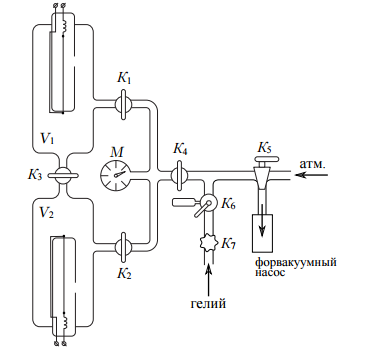
\includegraphics[width=0.9\textwidth]{thestation.png}
\end{center}
\caption{Схема установки}
\end {figure}
\begin{equation*}
{V}_{1}=360 \pm 0.5 \textup{ см}^3
\end{equation*}
\begin{equation*}
{V}_{2}=360 \pm 0.5 \textup{ см}^3
\end{equation*}
\begin{equation*}
\text{Погонная плотность: }\frac{L}{S}=7.0 \pm 0.5 \frac{1}{\textup{см}}
\end{equation*}
\newpage

\section{Работа и измерения}

\subsection{Начальные условия}

\noindent Максимальная откачка: $P_{0}=102.5 \text{ дел}$\\*
Расcчитаем сколько торр в одном делении: \\
\begin{enumerate}
	

\item Всего торр: $P_{0}=1.025 \text{ } \frac{\text{кгс}}{\text{см}^2} = 100.5181\cdot10^3\text{ Па} = 
753.95 \text{ торр}$
\item В одном делении 980,665 Па = 7.356 торр
\item Основные погрешности:
\end{enumerate}
$$\sigma_{V_1 + V_2} = \sqrt{\sigma_{V_1}^2 + \sigma_{V_2}^2 } = \sqrt{0.5^2 + 0.5^2} = 0.71 \textup{ см}^3$$
$$V_{\text{п}} = \dfrac{V_1 \cdot V_2}{V_1 + V_2}\text{; } \sigma_{V_{\text{п}}} =V_{\text{п}} \cdot
\sqrt{\Big(\dfrac{\sigma_{V_{1}}}{V_{1}}\Big)^{2}+\Big(\dfrac{\sigma_{V_{2}}}{V_{2}}\Big)^{2}+\Big(\dfrac{\sigma_{V_{1}+V_{2}}}{V_{1}+V_{2}}\Big)^{2}}=$$
$$=180\cdot\sqrt{\Big(\dfrac{0.5}{360}\Big)^{2}+\Big(\dfrac{0.5}{360}\Big)^{2}+\Big(\dfrac{0.71}{720}\Big)^{2}} = 0.396 \textup{ см}^3$$

\newpage

\subsection{Измерения при 40 торр}

1. Давление, полученное при открытии кранов К1, К2, К3: $P_{\Sigma } = 47.814 \text{ торр}$

\begin{table}[H]
	\centering
		\caption{измерения при рабочем давлении 40 торр}
	\begin{tabu} to 0.8\textwidth {| X[c] | X[c] | X[c] |}
		\hline
		$t, \text{ с}$ & \text{значение} & \text{логарифм} \\ \hline \hline
		0.00 & 255.0 & 0.000    \\ \hline
		6.35 & 250.7 & 0.017    \\ \hline
		12.70 & 244.3 & 0.043    \\ \hline
		19.04 & 237.0 & 0.073    \\ \hline
		25.39 & 229.6 & 0.105    \\ \hline
		31.74 & 223.3 & 0.133    \\ \hline
		38.09 & 216.0 & 0.166    \\ \hline
		44.43 & 210.6 & 0.191    \\ \hline
		50.78 & 204.2 & 0.222    \\ \hline
		57.13 & 191.7 & 0.254    \\ \hline
		63.48 & 192.5 & 0.281    \\ \hline
		69.83 & 186.2 & 0.315    \\ \hline
		76.17 & 180.8 & 0.344    \\ \hline
		82.52 & 175.5 & 0.374    \\ \hline
		88.87 & 171.0 & 0.400   \\ \hline
		95.22 & 165.8 & 0.431    \\ \hline
 		101.57 & 161.4 & 0.457    \\ \hline
		107.91 & 156.1 & 0.491    \\ \hline
		114.26 & 151.7 & 0.519    \\ \hline
		120.61 & 147.4 & 0.548    \\ \hline
		126.96 & 143.0 & 0.578    \\ \hline 
		133.30 & 139.0 & 0.607    \\ \hline 
		139.65 & 165.0 & 0.636    \\ \hline 
		146.00 & 131.0 & 0.666    \\ \hline 
	\end{tabu}

\end{table}

2. Рассчитаем коэффициент наклона графика с помощью МНК:\\

\begin{equation*}
k = \frac{\langle xy \rangle - \langle x \rangle \langle y \rangle}{\langle x^2 \rangle - \langle x \rangle ^ 2} = 4.65 \cdot 10^{-3} \text{ ;}
\end{equation*}


$$  \sigma_{k} = 0.03 \cdot 10^{-3}$$






3. Расчитаем коэффициент взаимной диффузии:

$$k = 1 / {\tau} = \dfrac{V_1 + V_2}{V_1 \cdot V_2} \cdot \dfrac{S\cdot D}{l}$$
\begin{equation}
D = k \cdot \dfrac{l}{S} \cdot \dfrac{V_1 \cdot V_2}{V_1 + V_2} = 0.00465 \cdot 7.0 \cdot \dfrac{360\cdot 360}{360+360} = 5.86  \text{ } \dfrac{\textup{см}^2}{\textup{с}}
\end{equation}

\begin {figure}[H]
\begin{center}
	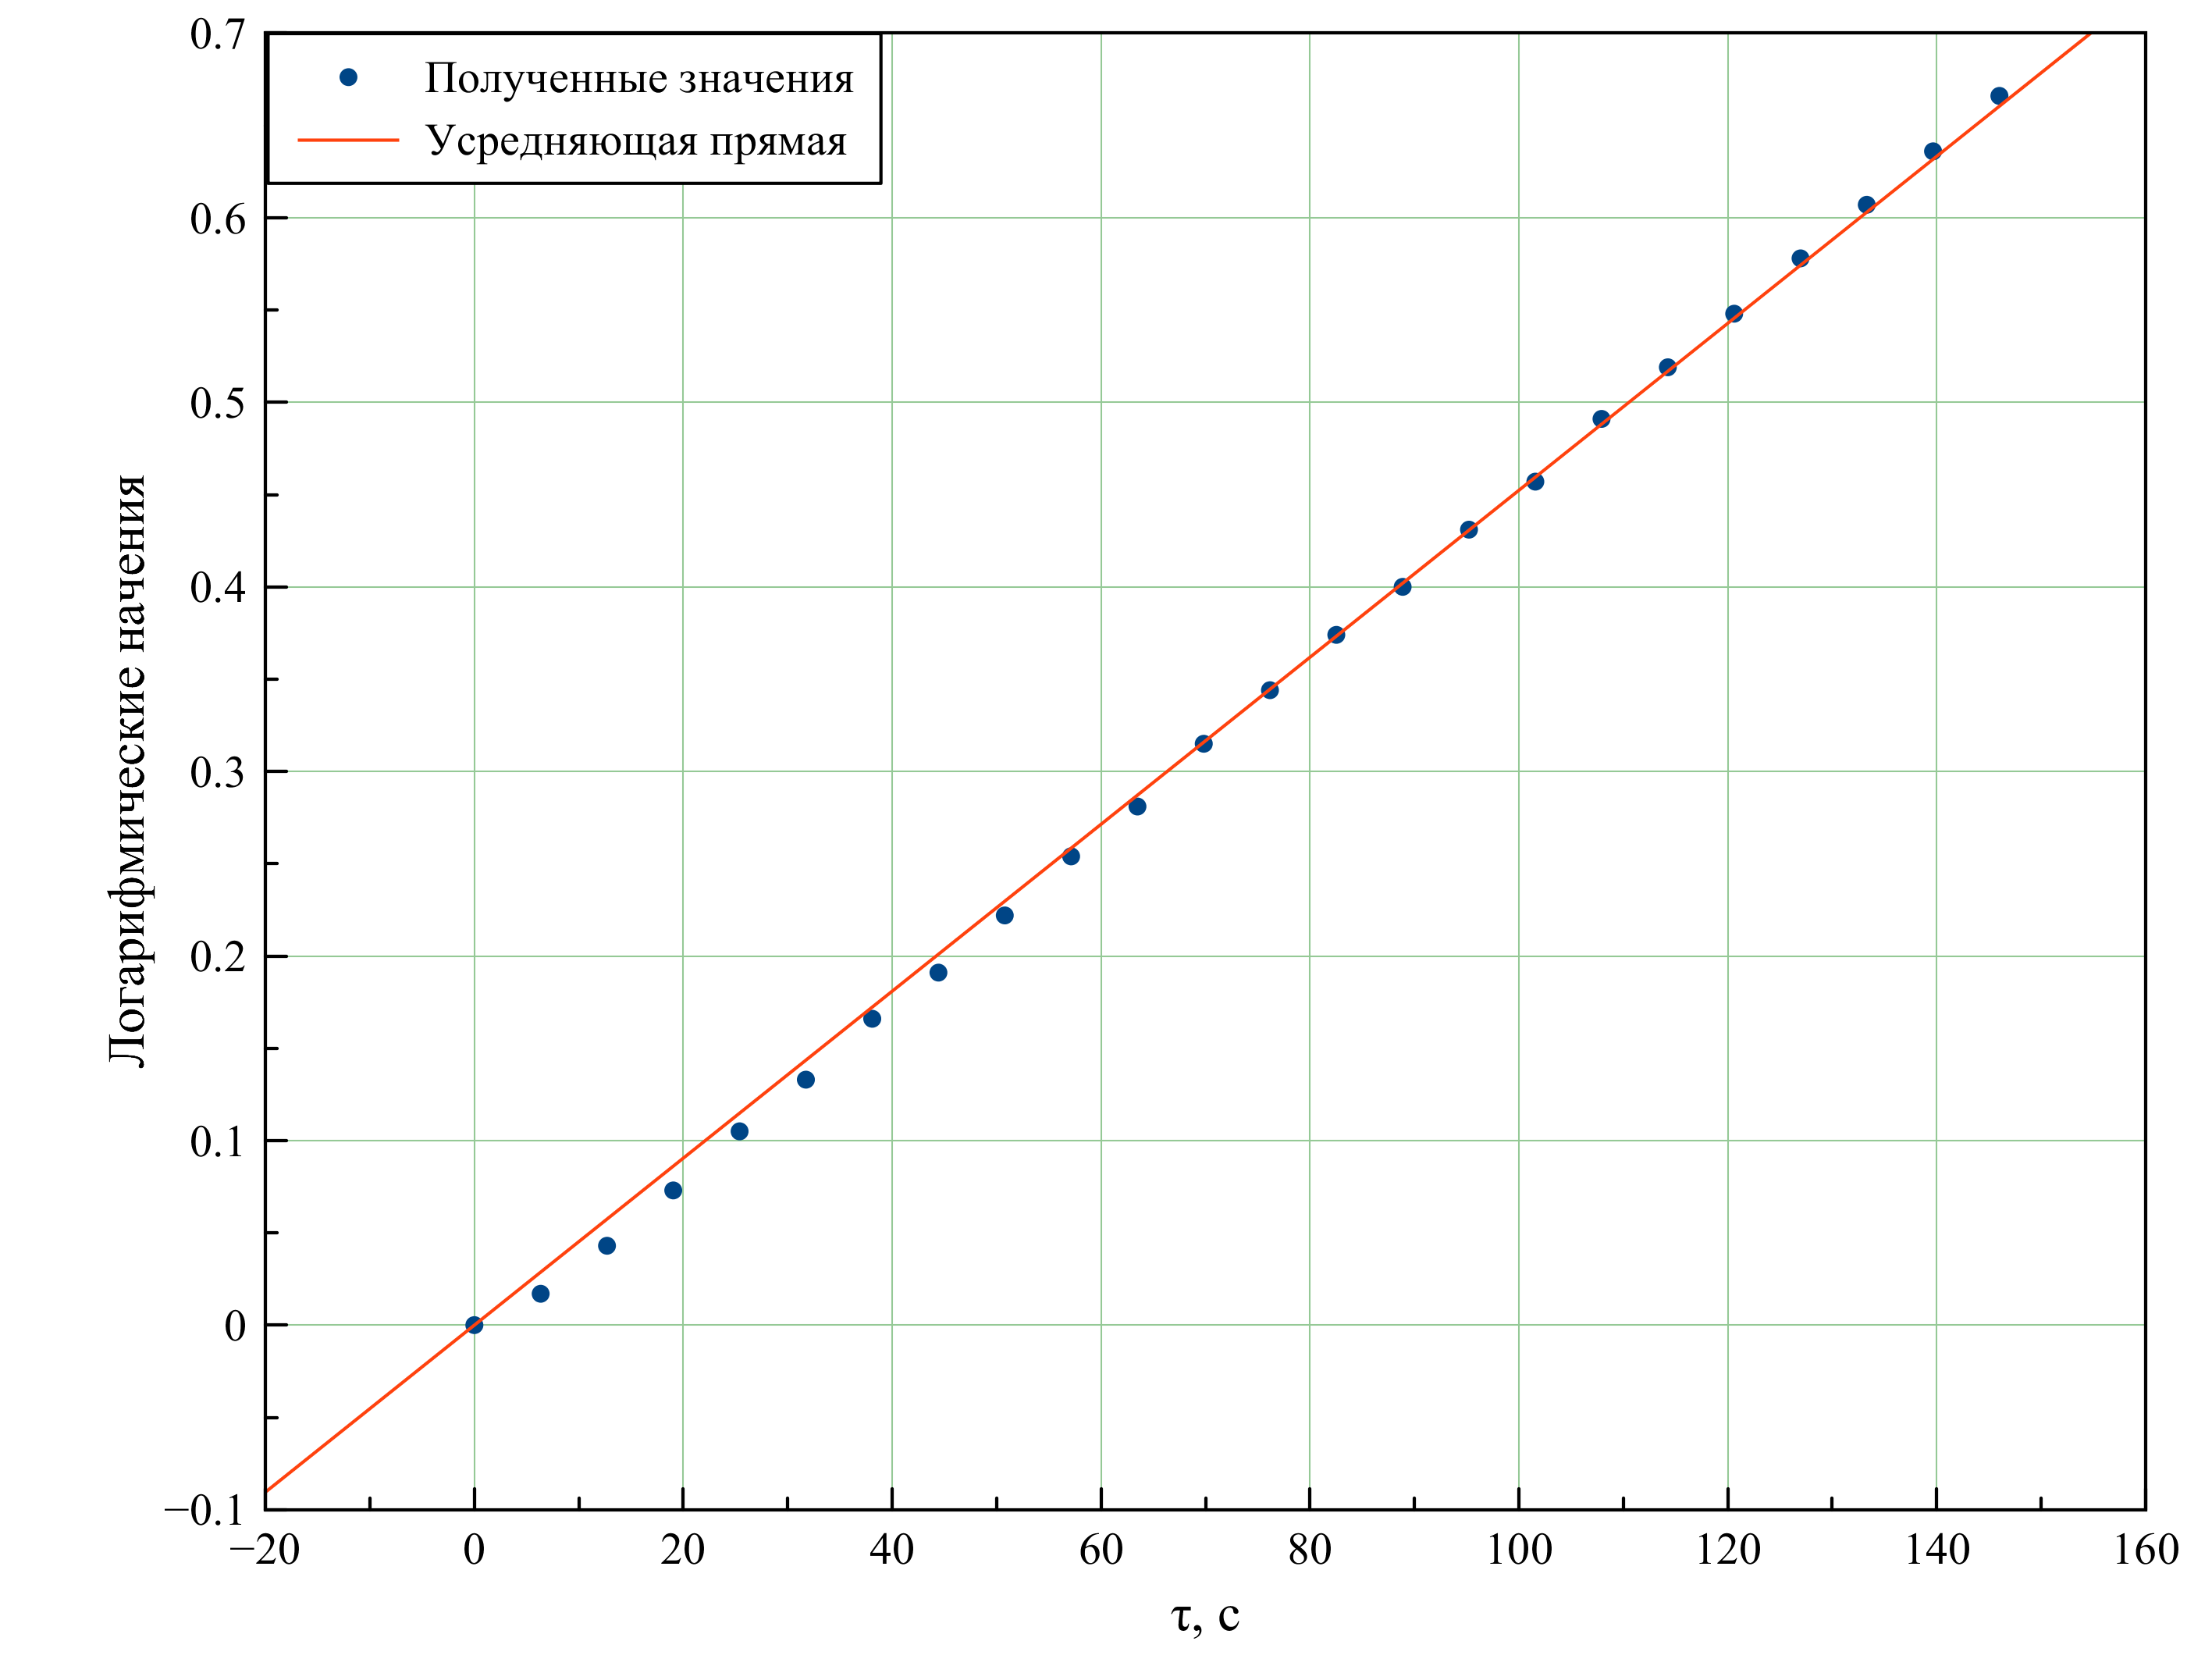
\includegraphics[width=1.0\textwidth]{graph1.png}
\end{center}
\caption{график при рабочем давлении 40 торр}
\end {figure}
 \begin{equation}
\sigma_{D} = D \cdot \sqrt{\Big(\dfrac{\sigma_{k}}{k}\Big)^{2} + 
\Big(\dfrac{\sigma_{\nicefrac{l}{S}}}{\nicefrac{l}{S}}\Big)^{2}+\Big(\dfrac{\sigma_{V_\text{п}}}{V_\text{п}}\Big)^{2}} 
\end{equation}
$$\sigma_{D}= 5.86 \cdot \sqrt{\Big(\dfrac{0.00003}{0.00465}\Big)^{2} + \Big(\dfrac{0.5}{7.0}\Big)^{2} + \Big(\dfrac{0.396}{180}\Big)^{2}} = 0.42 \text{ } \dfrac{\textup{см}^2}{\textup{с}}$$
%\end{equation}
\Large  В итоге получим: $ D_1 = 5.86 \pm 0.42 \text{ }\dfrac{\textup{см}^2}{\textup{с}} $
\normalsize
\newpage

\subsection{Измерения при 100 торр}

Давление, полученное при открытии кранов К1, К2, К3: $P_{\Sigma } = 94.5 \text{ торр}$

\begin{table}[H]
	\centering
	\begin{tabu} to 0.6\textheight {| X[c] | X[c] | X[c] |}
		\hline
		$t, \text{ с}$ & \text{значение} & \text{логарифм} \\ \hline %\hline
		0.00 & 255.0 & 0.000    \\ \hline
		6.61 & 252.0 & 0.012    \\ \hline
		13.22 & 249.0 & 0.024    \\ \hline
		19.83 & 246.2 & 0.035    \\ \hline
		26.43 & 244.0 & 0.044    \\ \hline
		33.04 & 241.0 & 0.057    \\ 
		\hline
		39.65 & 238.3 & 0.068    \\ 
		\hline
		46.26 & 235.7 & 0.079    \\ 
		\hline
		52.87 & 233.0 & 0.090    \\ 
		\hline
		59.48 & 230.5 & 0.101    \\ 
		\hline
		66.09 & 228.0 & 0.112    \\ 
		\hline
		72.70 & 225.3 & 0.124    \\ 
		\hline
		79.30 & 223.0 & 0.134    \\ 
		\hline
		85.91 & 221.0 & 0.143    \\ 
		\hline
		92.53 & 218.5 & 0.155    \\ 
		\hline
		99.13 & 216.0 & 0.166    \\ 
		\hline
		105.74 & 214.0 & 0.175    \\ 
		\hline
		112.35 & 211.7 & 0.186    \\ 
		\hline
		118.96 & 209.0 & 0.199    \\ 
		\hline
		125.57 & 207.0 & 0.209    \\ 
		\hline
		132.17 & 205.0 & 0.218    \\ 
		\hline
		138.78 & 203.0 & 0.228    \\ 
		\hline
		145.39 & 201.0 & 0.238    \\ 
		\hline
		152.00 & 199.0 & 0.248    \\ 
		\hline
	\end{tabu}
	\caption{измерения при рабочем давлении 100 торр}
\end{table}

2. Рассчитаем коэффициент наклона графика с помощью МНК:\\

\begin{equation*}
k = \frac{\langle xy \rangle - \langle x \rangle \langle y \rangle}{\langle x^2 \rangle - \langle x \rangle ^ 2} = 1.55 \cdot 10^{-3} \text{ ;}
\end{equation*}


$$  \sigma_{k} = 0.09 \cdot 10^{-3}$$


3. Расчитаем коэффициент взаимной диффузии по формулам (1) и (2): 

$$D = 0.00155 \cdot 7.0 \cdot \dfrac{360\cdot 360}{360+360} = 1.96  \text{ } \dfrac{\textup{см}^2}{\textup{с}}   \text{ ;}$$
$$\sigma_D =  1.96 \cdot \sqrt{\Big(\dfrac{0.00009}{0.00155}\Big)^{2} + \Big(\dfrac{0.5}{7.0}\Big)^{2} + \Big(\dfrac{0.396}{180}\Big)^{2}} = 0.18 \text{ } \dfrac{\textup{см}^2}{\textup{с}}$$
\Large  В итоге получим: $ D_1 = 1.96 \pm 0.18 \text{ } \dfrac{\textup{см}^2}{\textup{с}} $
\normalsize
\begin {figure}[H]
\begin{center}
	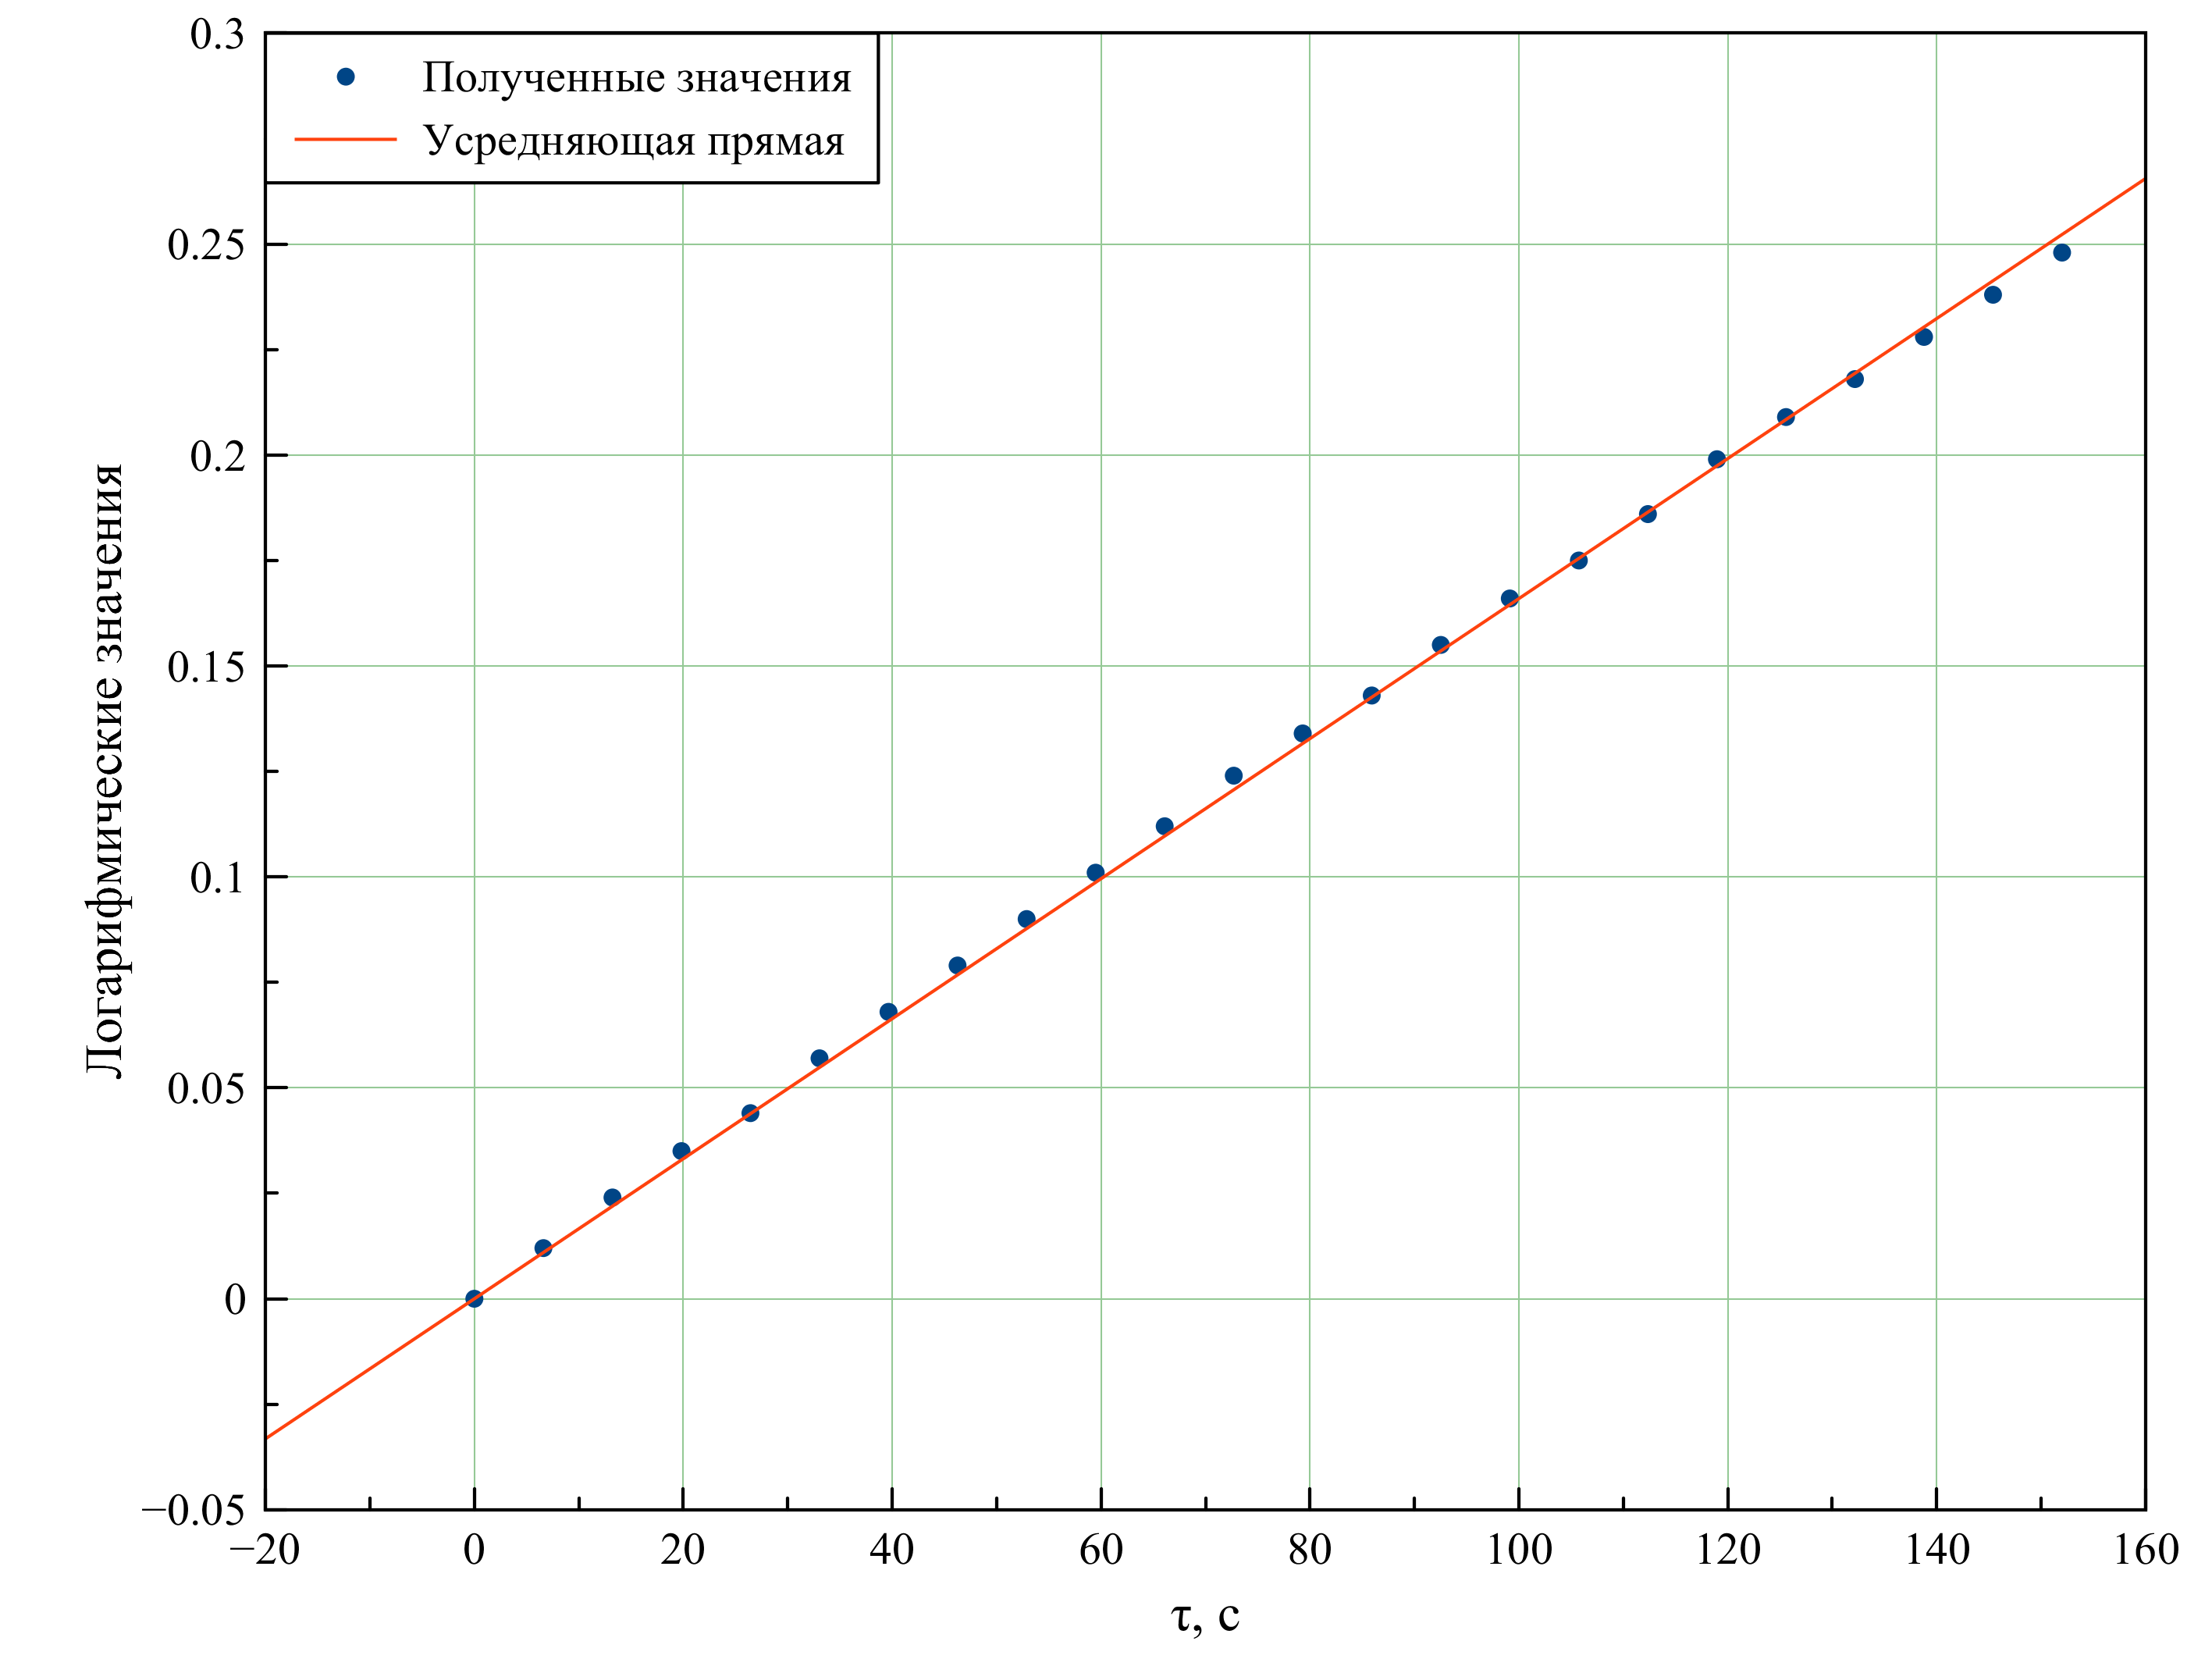
\includegraphics[width=1.0\textwidth]{graph2.png}
\end{center}
\caption{график при рабочем давлении 100 торр}
\end {figure}



\newpage

\subsection{Измерения при 150 торр}

Давление, полученное при открытии кранов К1, К2, К3: $P_{\Sigma } = 142.86 \text{ торр}$

\begin{table}[H]
	\centering
	\begin{tabu} to 0.6\textheight {| X[c] | X[c] | X[c] |}
		\hline
		$t, \text{ с}$ & \text{значение} & \text{логарифм} \\ \hline \hline
		0.00 & 255.0 & 0.000    \\ 
		\hline
		6.53 & 251.0 & 0.016    \\ 
		\hline
		13.05 & 248.9 & 0.025    \\ 
		\hline
		19.57 & 246.0 & 0.038   \\ 
		\hline
		26.09 & 243.9 & 0.047    \\ 
		\hline
		32.61 & 241.3 & 0.058    \\ 
		\hline
		39.13 & 240.0 & 0.064    \\ 
		\hline
		45.66 & 238.0 & 0.073    \\ 
		\hline
		52.18 & 236.0 & 0.082    \\ 
		\hline
		58.70 & 234.3 & 0.090  \\ 
		\hline
		65.22 & 232.0 & 0.100    \\ 
		\hline
		71.74 & 231.0 & 0.105    \\ 
		\hline
		78.26 & 228.7 & 0.116    \\ 
		\hline
		84.79 & 226.2 & 0.128    \\ 
		\hline
		91.31 & 225.0 & 0.133    \\ 
		\hline
		97.83 & 223.1 & 0.142    \\ 
		\hline
		104.35 & 222.0 & 0.148    \\ 
		\hline
		110.87 & 220.0 & 0.157    \\ 
		\hline
		117.39 & 218.0 & 0.167    \\ 
		\hline
		123.92 & 216.0 & 0.177    \\ 
		\hline
		130.44 & 214.0 & 0.187    \\ 
		\hline
		136.96 & 212.0 & 0.197    \\ 
		\hline
	\end{tabu}
	\caption{измерения при рабочем давлении 150 торр}
\end{table}

2. Рассчитаем коэффициент наклона графика с помощью МНК:\\

\begin{equation*}
k = \frac{\langle xy \rangle - \langle x \rangle \langle y \rangle}{\langle x^2 \rangle - \langle x \rangle ^ 2} = 1.36 \cdot 10^{-3} \text{ ;}
\end{equation*}


$$  \sigma_{k} = 0.01 \cdot 10^{-3}$$

3. Расчитаем коэффициент взаимной диффузии по формулам (1) и (2): 

$$D = 0.00136 \cdot 7.0 \cdot \dfrac{360\cdot 360}{360+360} = 1.72  \text{ } \dfrac{\textup{см}^2}{\textup{с}}   \text{ ;}$$
$$\sigma_D =  1.72 \cdot \sqrt{\Big(\dfrac{0.00001}{0.00136}\Big)^{2} + \Big(\dfrac{0.5}{7.0}\Big)^{2} + \Big(\dfrac{0.396}{180}\Big)^{2}} = 0.12 \text{ } \dfrac{\textup{см}^2}{\textup{с}}$$
\Large  В итоге получим: $ D_1 = 1.72 \pm 0.12 \text{ } \dfrac{\textup{см}^2}{\textup{с}} $
\normalsize
\begin {figure}[H]
\begin{center}
	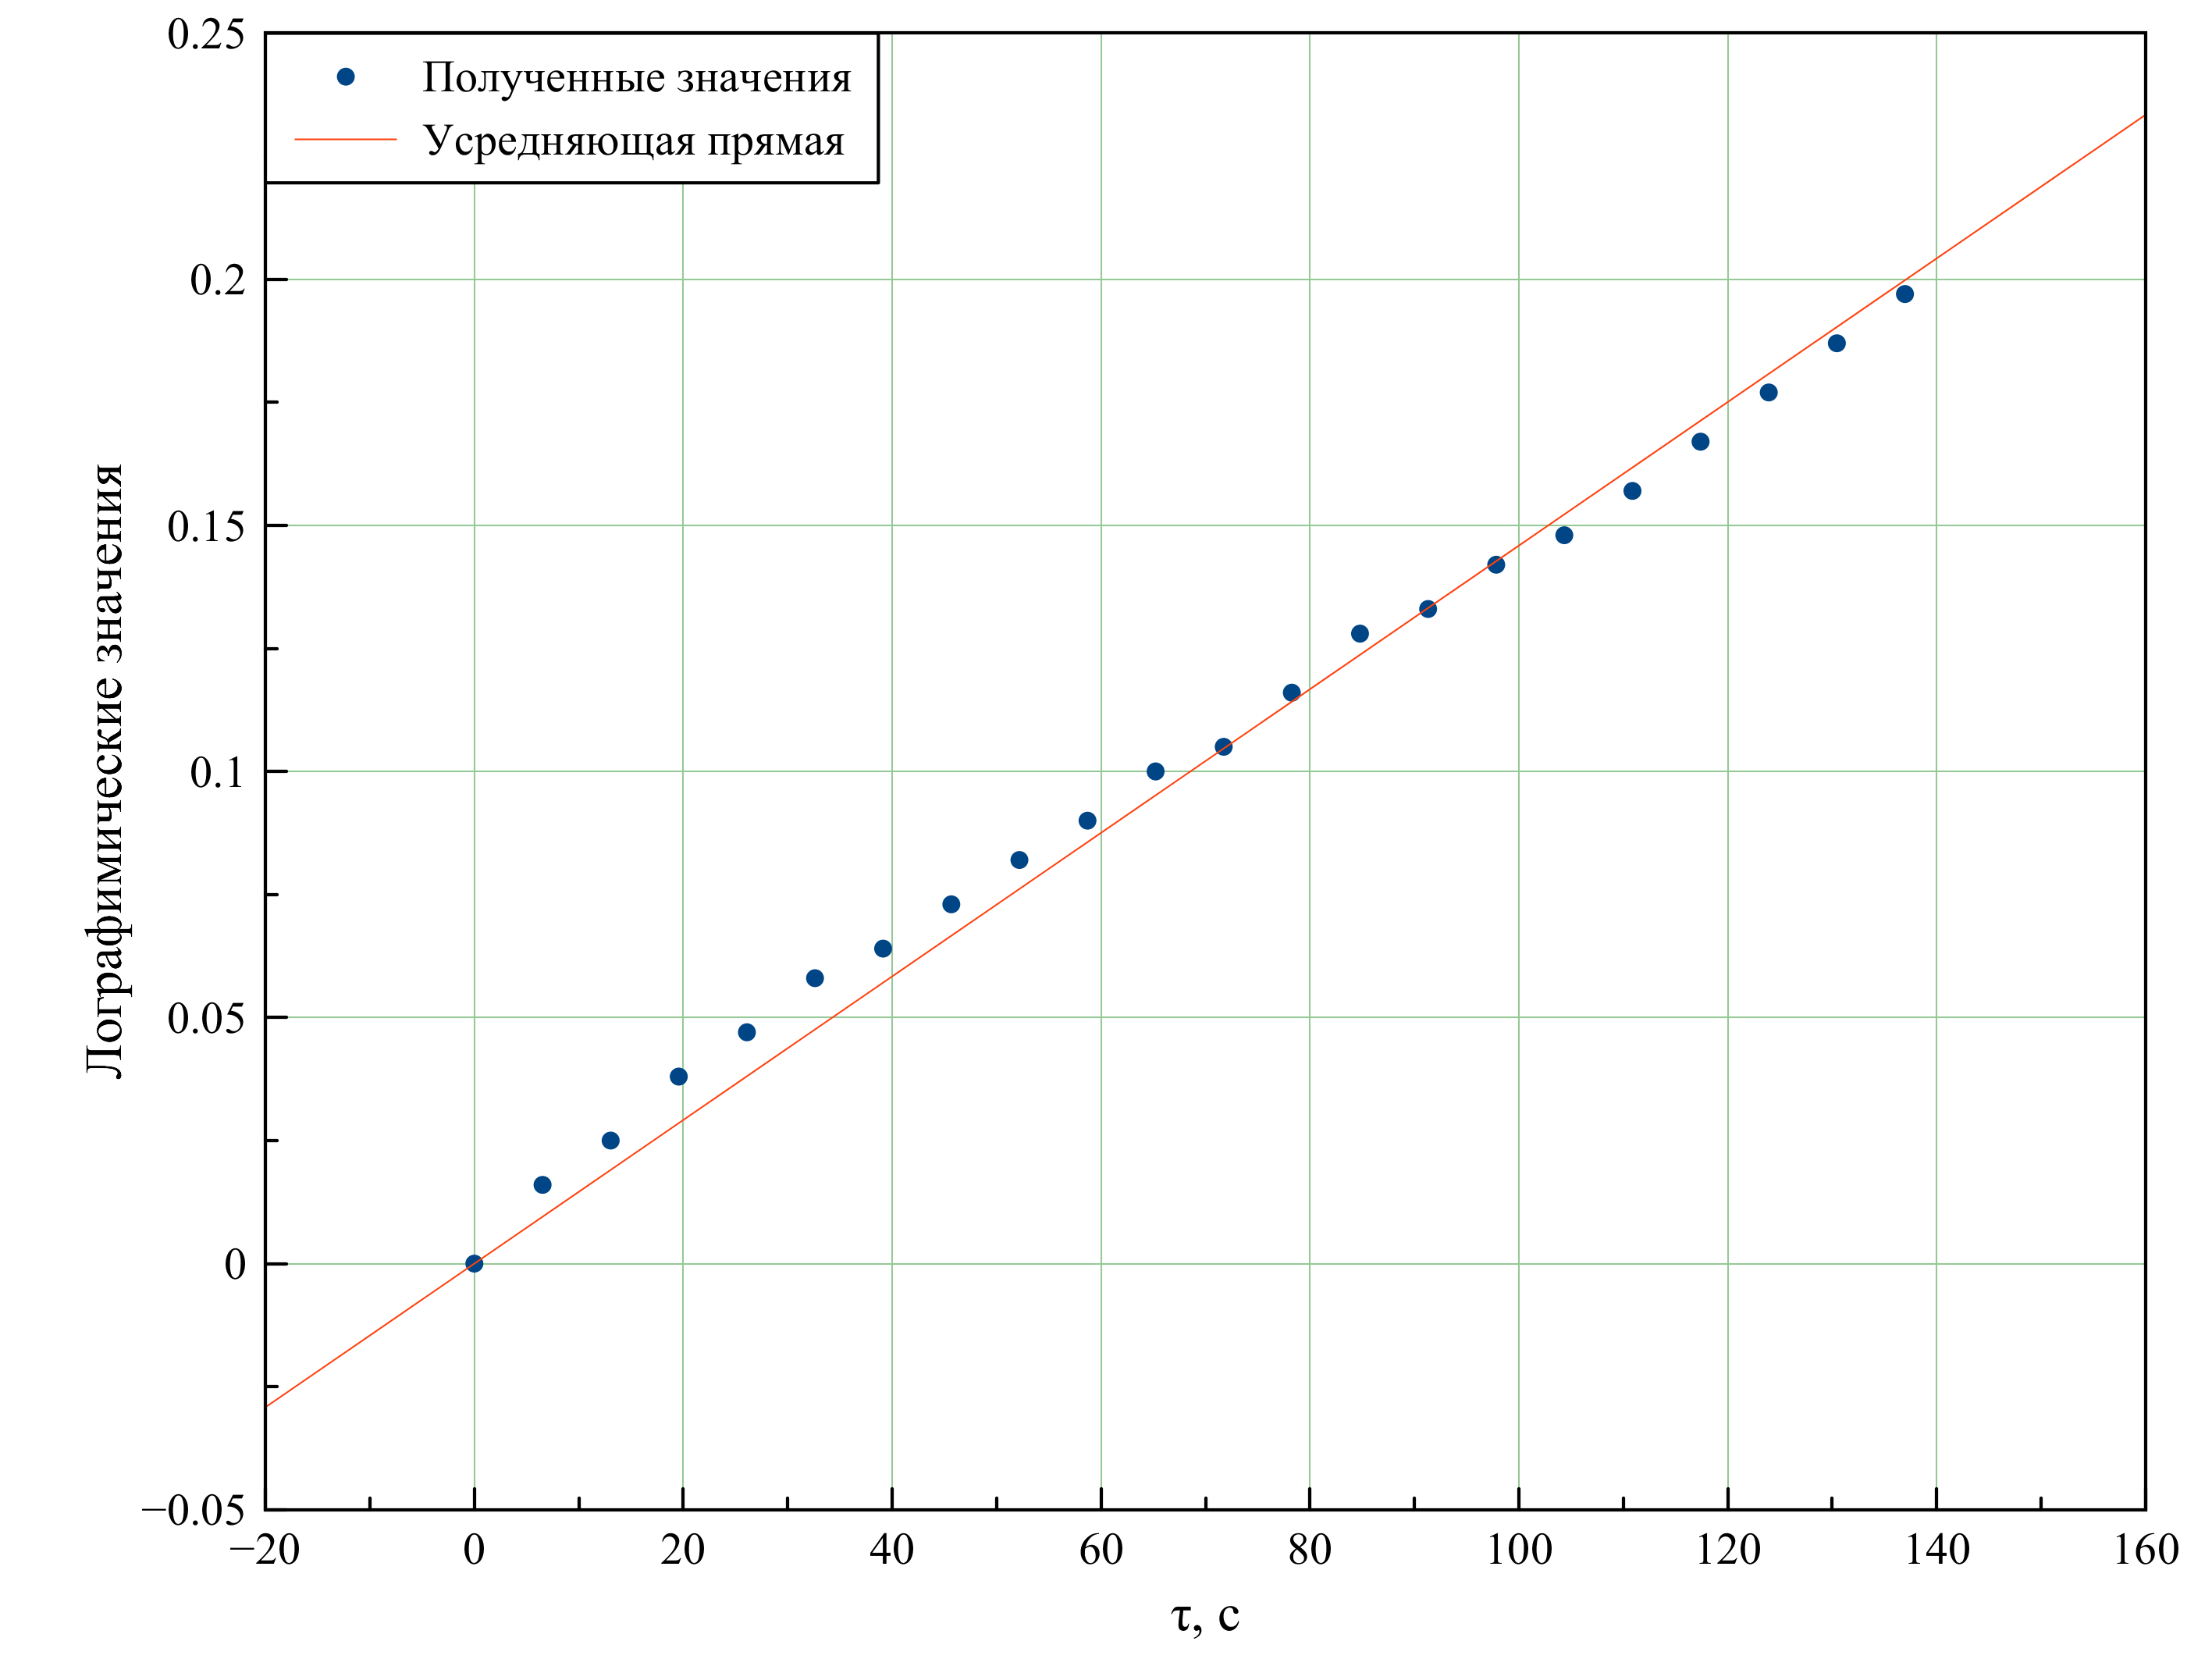
\includegraphics[width=1.0\textwidth]{graph3.png}
\end{center}
\caption{график при рабочем давлении 150 торр}
\end {figure}

\newpage

\subsection{Измерения при 200 торр}

Давление, полученное при открытии кранов К1, К2, К3: $P_{\Sigma } = 176.54 \text{ торр}$

\begin{table}[H]
	\centering
	\begin{tabu} to 0.6\textheight {| X[c] | X[c] | X[c] |}
		\hline
		$t, \text{ с}$ & \text{значение} & \text{логарифм} \\ \hline \hline
		0.00 & 255.0 & 0.000    \\ 
		\hline
		15.17 & 250.0  & 0.020     \\
		 \hline
		30.35 & 245.0  & 0.040     \\
		\hline
		45.52 & 240.5  & 0.059     \\
		\hline
		60.70 & 235.3  & 0.080     \\
		\hline
		75.87 & 231.0  & 0.099     \\
		\hline
		91.04 & 226.0  & 0.121    \\
		\hline
		106.22 & 221.8  & 0.140     \\
		\hline
		121.39 & 217.6  & 0.159     \\
		\hline
		136.57 & 213.0  & 0.180     \\
		\hline
		151.74 & 209.0  & 0.199     \\
		\hline
		166.91 & 205.0  & 0.218     \\
		\hline
		182.09 & 200.9  & 0.238     \\
		\hline
		197.26 & 197.0  & 0.258     \\
		\hline
		212.43 & 193.0  & 0.279     \\
		\hline
		227.61 & 189.0  & 0.300     \\
		\hline
		242.78 & 185.2  & 0.320     \\
		\hline
		257.96 & 182.0  & 0.337     \\
		\hline
		273.13 & 178.0  & 0.359     \\
		\hline
		288.30 & 175.0  & 0.376     \\
		\hline
		303.48 & 172.0  & 0.394     \\
		\hline
		318.65 & 168.3  & 0.415     \\
		\hline
		333.83 & 161.0  & 0.460     \\
		\hline
		349.00 & 118.0  & 0.771     \\
		\hline
	\end{tabu}
	\caption{измерения при рабочем давлении 200 торр}
\end{table}

2. Рассчитаем коэффициент наклона графика с помощью МНК:\\

\begin{equation*}
k = \frac{\langle xy \rangle - \langle x \rangle \langle y \rangle}{\langle x^2 \rangle - \langle x \rangle ^ 2} = 1.46 \cdot 10^{-3} \text{ ;}
\end{equation*}


$$  \sigma_{k} = 0.23 \cdot 10^{-3}$$

3. Расчитаем коэффициент взаимной диффузии по формулам (1) и (2): 

$$D = 0.00146 \cdot 7.0 \cdot \dfrac{360\cdot 360}{360+360} = 1.83 \text{ } \dfrac{\textup{см}^2}{\textup{с}}   \text{ ;}$$
$$\sigma_D =  1.73 \cdot \sqrt{\Big(\dfrac{0.00023}{0.00183}\Big)^{2} + \Big(\dfrac{0.5}{7.0}\Big)^{2} + \Big(\dfrac{0.396}{180}\Big)^{2}} = 0.32 \text{ } \dfrac{\textup{см}^2}{\textup{с}}$$
\Large  В итоге получим: $ D_1 = 1.83 \pm 0.32 \text{ } \dfrac{\textup{см}^2}{\textup{с}} $
\normalsize
\begin {figure}[H]
\begin{center}
	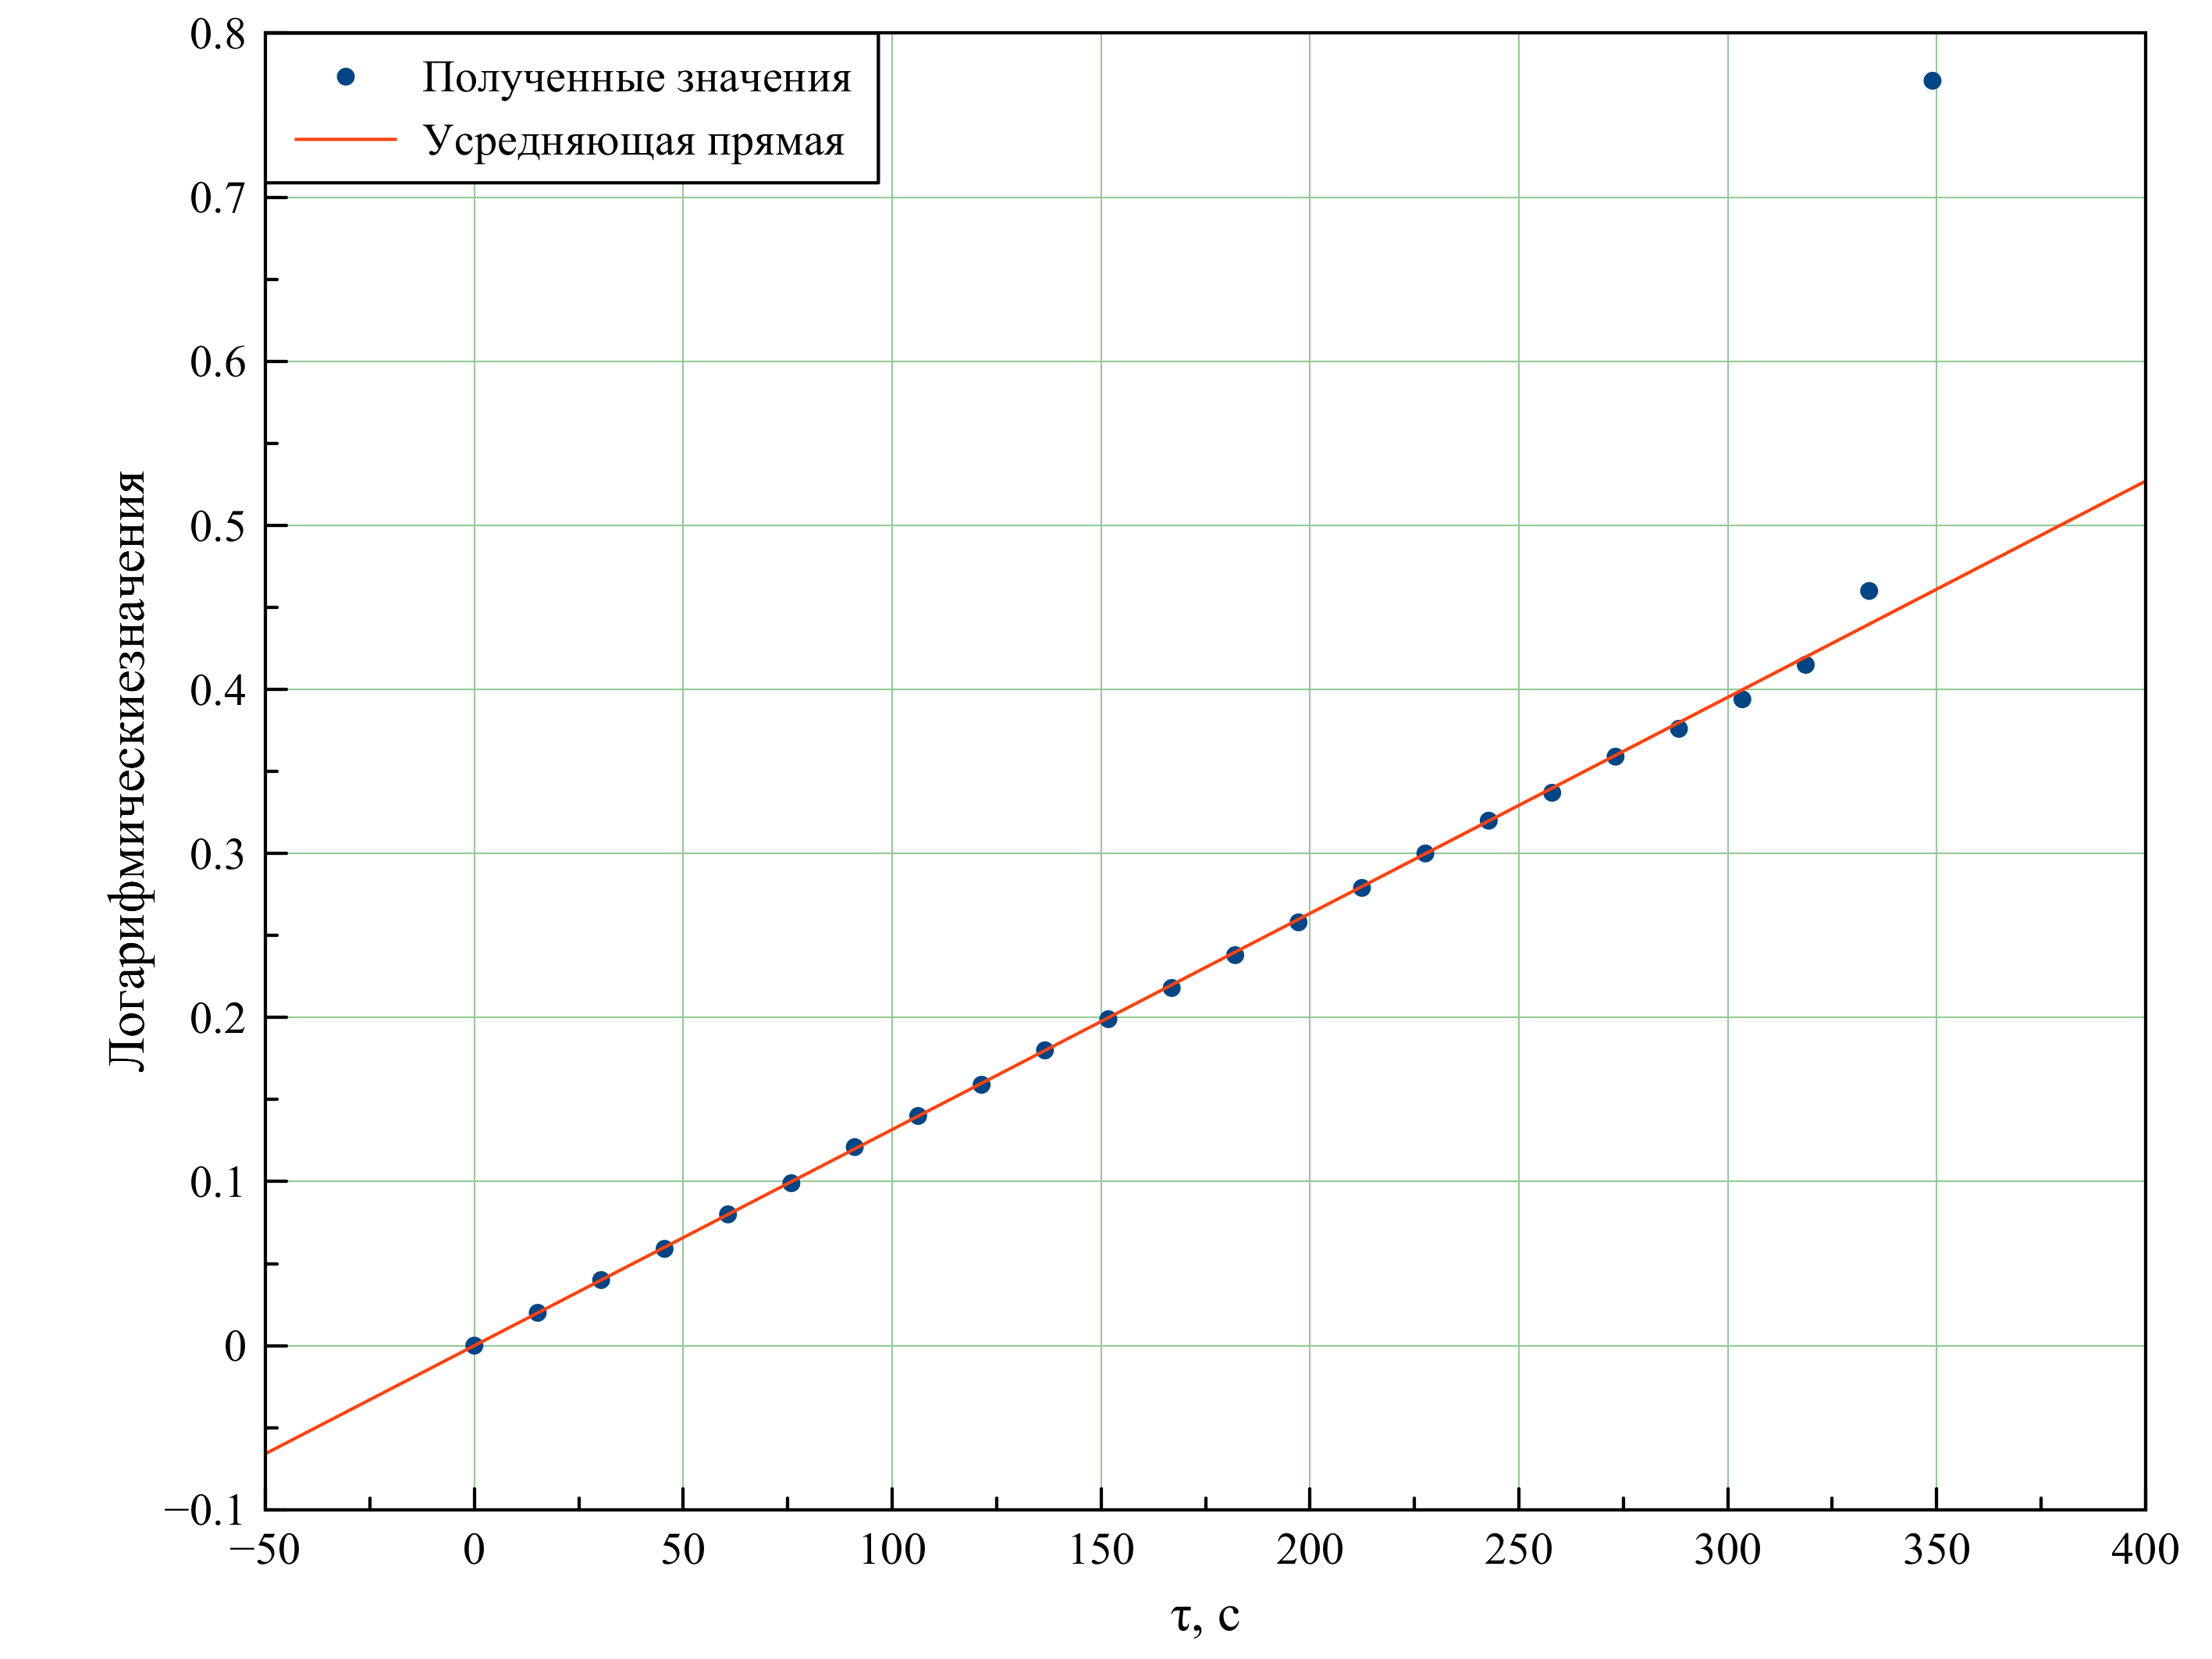
\includegraphics[width=1.0\textwidth]{graph4.png}
\end{center}
\caption{график при рабочем давлении 200 торр}
\end {figure}

\newpage

\subsection{Измерения при 300 торр}

Давление, полученное при открытии кранов К1, К2, К3: ${P}_{\Sigma} = 253.78 \text{ торр}$


\begin{table}[H]
	\centering
	\begin{tabu} to 0.6\textheight {|X[c]|X[c]|X[c]|}
		\hline
		$t, \text{ с}$ & \text{значение} & \text{логарифм} \\ \hline \hline
		0.00	&255.0	& 0.000 \\ \hline
		20.74	&248.5	& 0.030 \\ \hline
		41.48	&244.5	& 0.050 \\ \hline
		62.22	&239.5	& 0.074 \\ \hline
		82.95	&236.1	& 0.091 \\ \hline
		103.69	&231.5	& 0.114 \\ \hline
		124.43	&228.5	& 0.130 \\ \hline
		145.17	&224.5	& 0.151 \\ \hline
		165.91	&221.5	& 0.167 \\ \hline
		186.65	&217.5	& 0.189 \\ \hline
		207.39	&215.5	& 0.206 \\ \hline
		228.13	&211.5	& 0.223 \\ \hline
		248.87	&207.5	& 0.246 \\ \hline
		269.61	&204.5	& 0.264 \\ \hline
		290.35	&201.5	& 0.282 \\ \hline
		311.09	&198.5	& 0.301 \\ \hline
		331.82	&196.2	& 0.315 \\ \hline
		352.56	&193.5	& 0.333 \\ \hline
		373.30	&190.5	& 0.352 \\ \hline
		394.04  &187.5	& 0.372 \\ \hline
		414.78	&184.5	& 0.351 \\ \hline
		435.52	&182.5	& 0.405 \\ \hline
	\end{tabu}
\end{table}

2. Рассчитаем коэффициент наклона графика с помощью МНК:\\

\begin{equation*}
k = \frac{\langle xy \rangle - \langle x \rangle \langle y \rangle}{\langle x^2 \rangle - \langle x \rangle ^ 2} = 1.10 \cdot 10^{-3} \text{ ;}
\end{equation*}

$$  \sigma_{k} = 0.12 \cdot 10^{-3}$$

3. Расчитаем коэффициент взаимной диффузии по формулам (1) и (2):

$$D = 0.00110 \cdot 7.0 \cdot \dfrac{360\cdot 360}{360+360} = 1.39 \text{ } \dfrac{\textup{см}^2}{\textup{с}}   \text{ ;}$$
$$\sigma_D =  1.39 \cdot \sqrt{\Big(\dfrac{0.00012}{0.00110}\Big)^{2} + \Big(\dfrac{0.5}{7.0}\Big)^{2} + \Big(\dfrac{0.396}{180}\Big)^{2}} = 0.18 \text{ } \dfrac{\textup{см}^2}{\textup{с}}$$
\Large  В итоге получим: $ D_1 = 1.39 \pm 0.18 \text{ } \dfrac{\textup{см}^2}{\textup{с}} $
\normalsize

\begin {figure}[H]
\begin{center}
	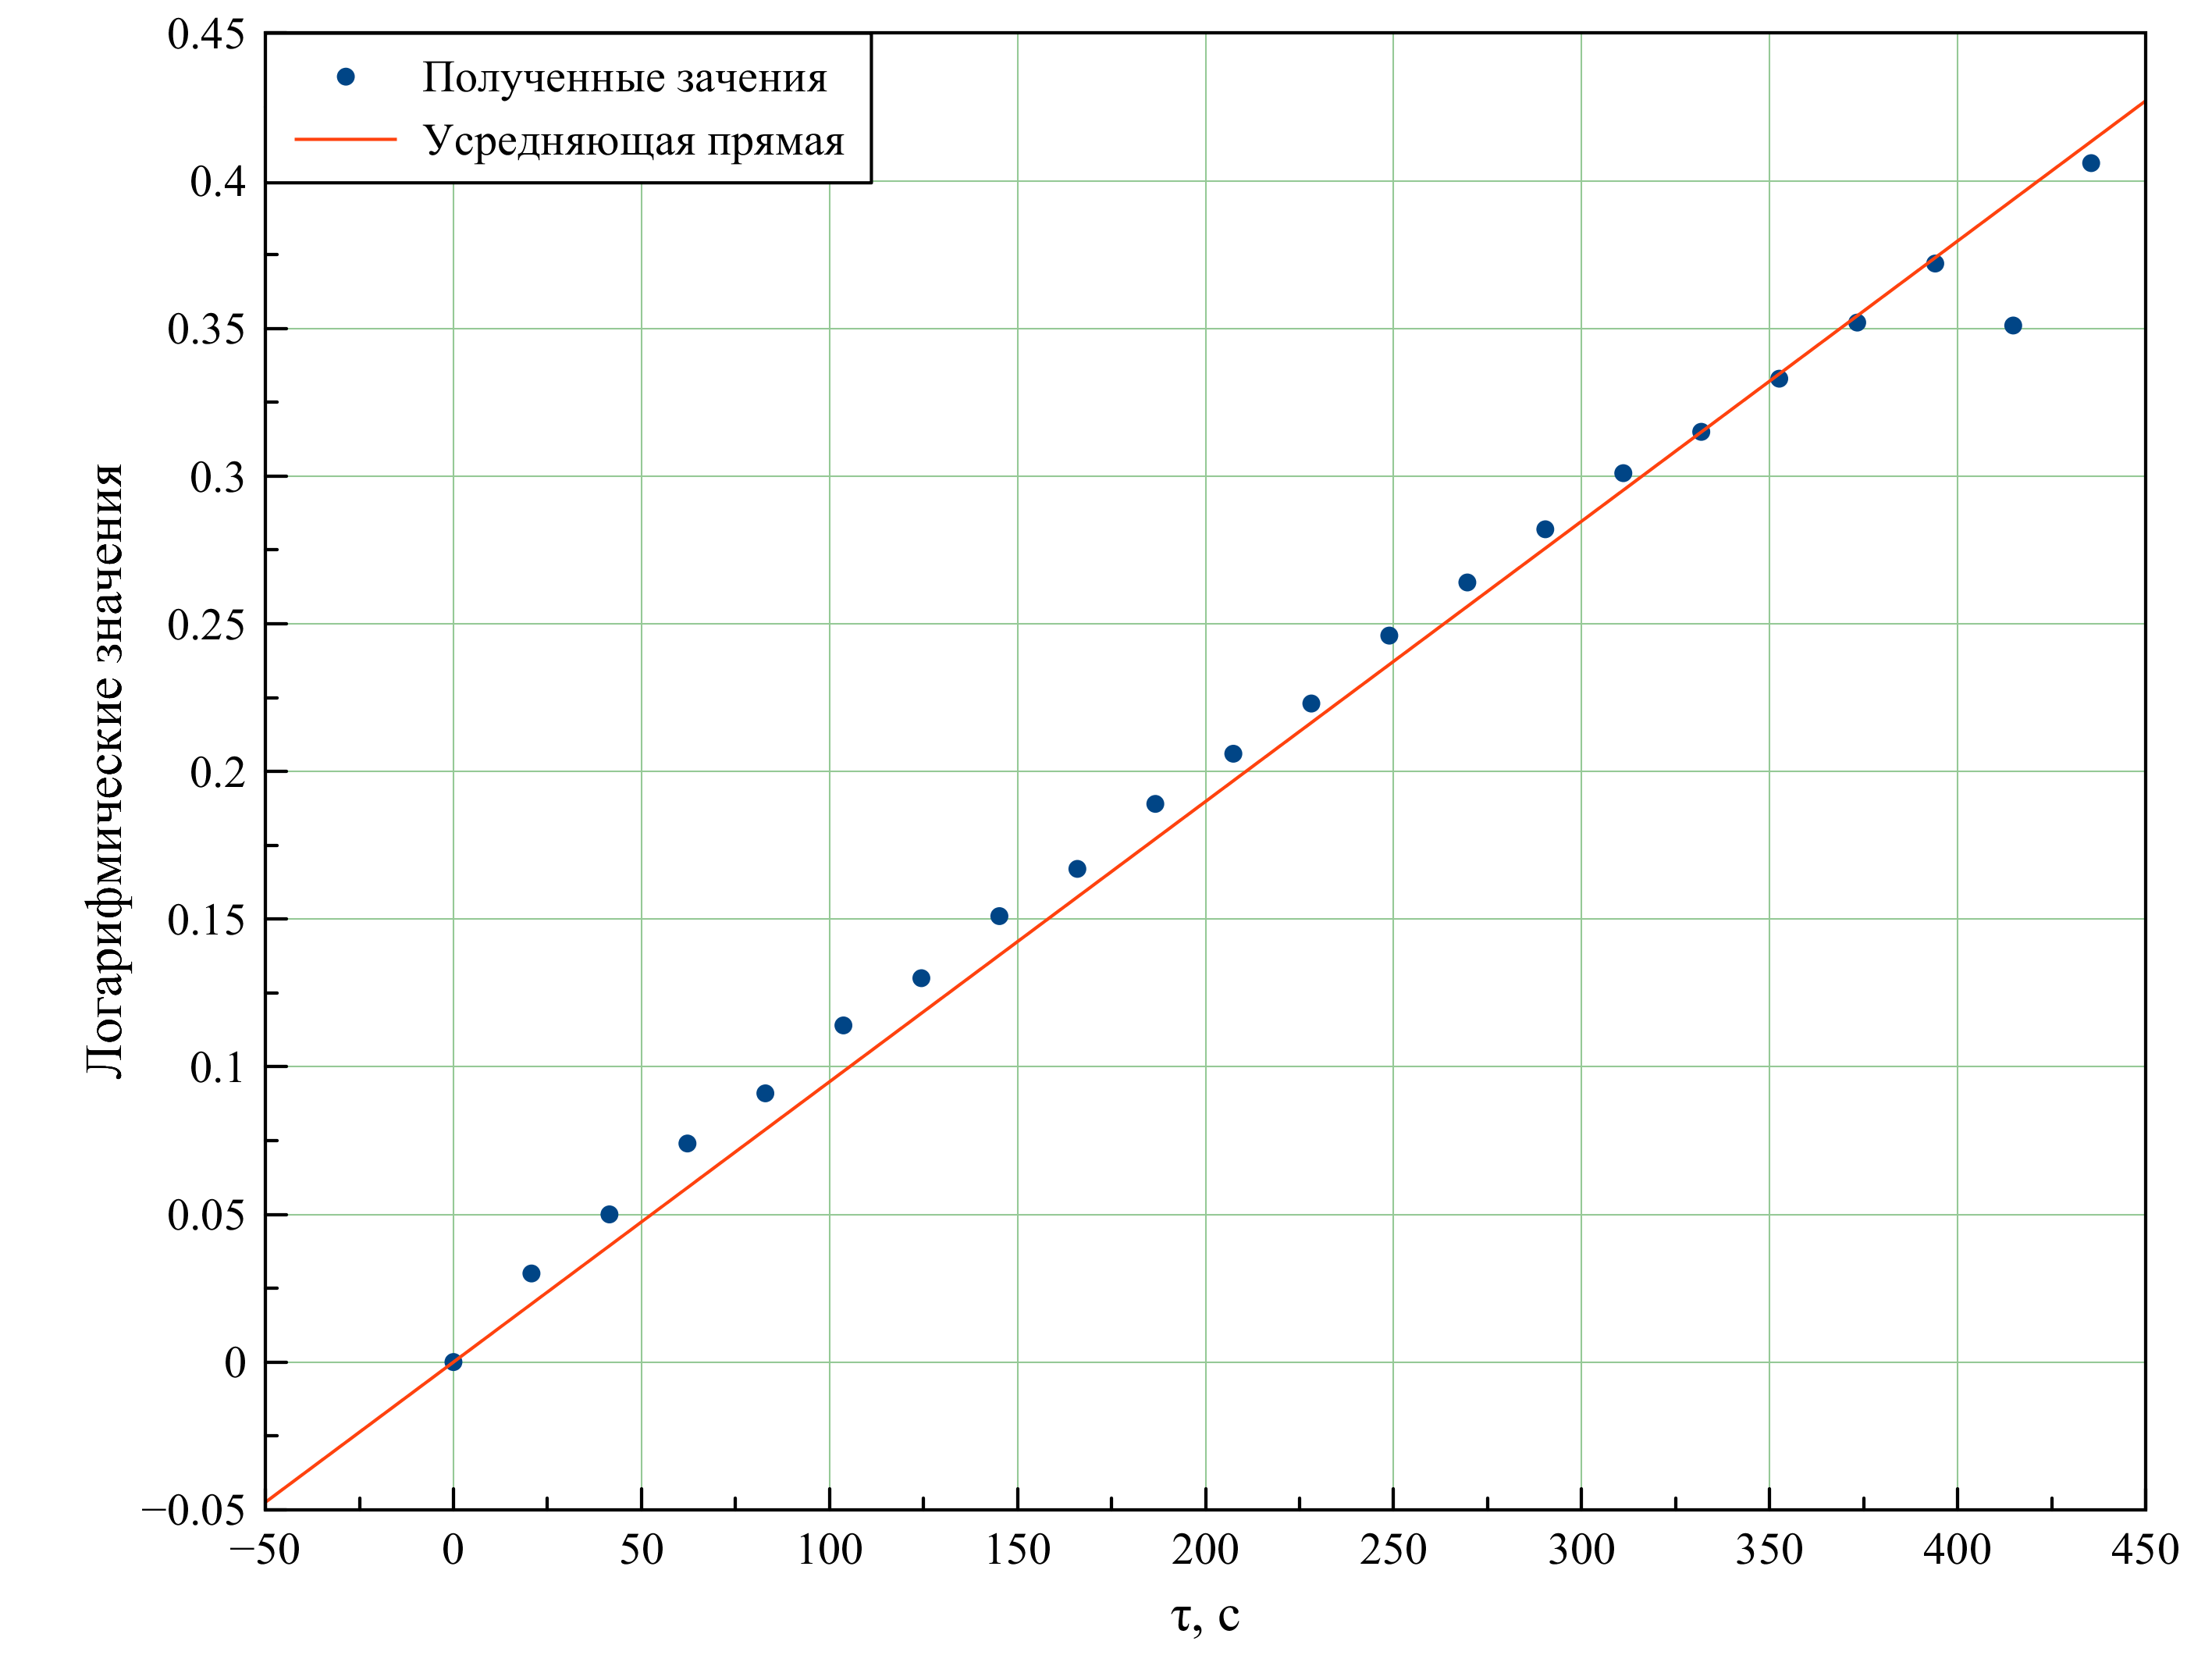
\includegraphics[width=1.0\textwidth]{graph5.png}
\end{center}
\caption{график при рабочем давлении 300 торр}
\end {figure}

\subsection{Коэффициент диффузии при атмосферном давлении}

\begin{table}[H]
		\begin{tabu} to 0.6\textheight {|X[c]|X[c]|X[c]|}
			\hline
			$D \text{, } \nicefrac{\textup{см}^2}{\textup{с}}$ & $P^{-1} \cdot 10^{3}  \text{, \nicefrac{1}{торр}}$ &  ${P}^{-1} \cdot 10^{5} \text{, \nicefrac{1}{Па}}$  \\ \hline \hline
	     	4.37 & 25.0 & 18.75	\\ \hline	
	     	2.08 & 10.0 & 7.50\\ \hline
	     	1.83 & 6.7 & 5.00\\ \hline
	     	1.66 & 5.0 & 3.75\\ \hline
	     	1.21 & 3.3 & 2.50\\ \hline		
		\end{tabu}
\end{table}

1. Рассчитаем с помощью МНК коэффициент наклона графика :
$$k = \dfrac{\langle x\cdot y \rangle - \langle x \rangle \cdot \langle y \rangle}{\langle x^2 \rangle - \langle x \rangle ^ {2}} = \dfrac{23.1875-7.5\cdot 2.23}{(90.625-7.5^2)\cdot 10^{-5}} = 18 799.9$$ 

$$\sigma_{k} = \dfrac{1}{\sqrt{n}} \cdot \sqrt{\dfrac{\langle y^2 \rangle - \langle y \rangle ^ {2}}{\langle x^2 \rangle - \langle x \rangle ^ {2}}-k^2} = \dfrac{1}{\sqrt{5}}\cdot \sqrt{\dfrac{6.198-2.23^2}{(90.625-7.5^2)\cdot10^{-10}}-18 799.9^2} = 875.1$$

\begin{figure}[H]
	\begin{center}
		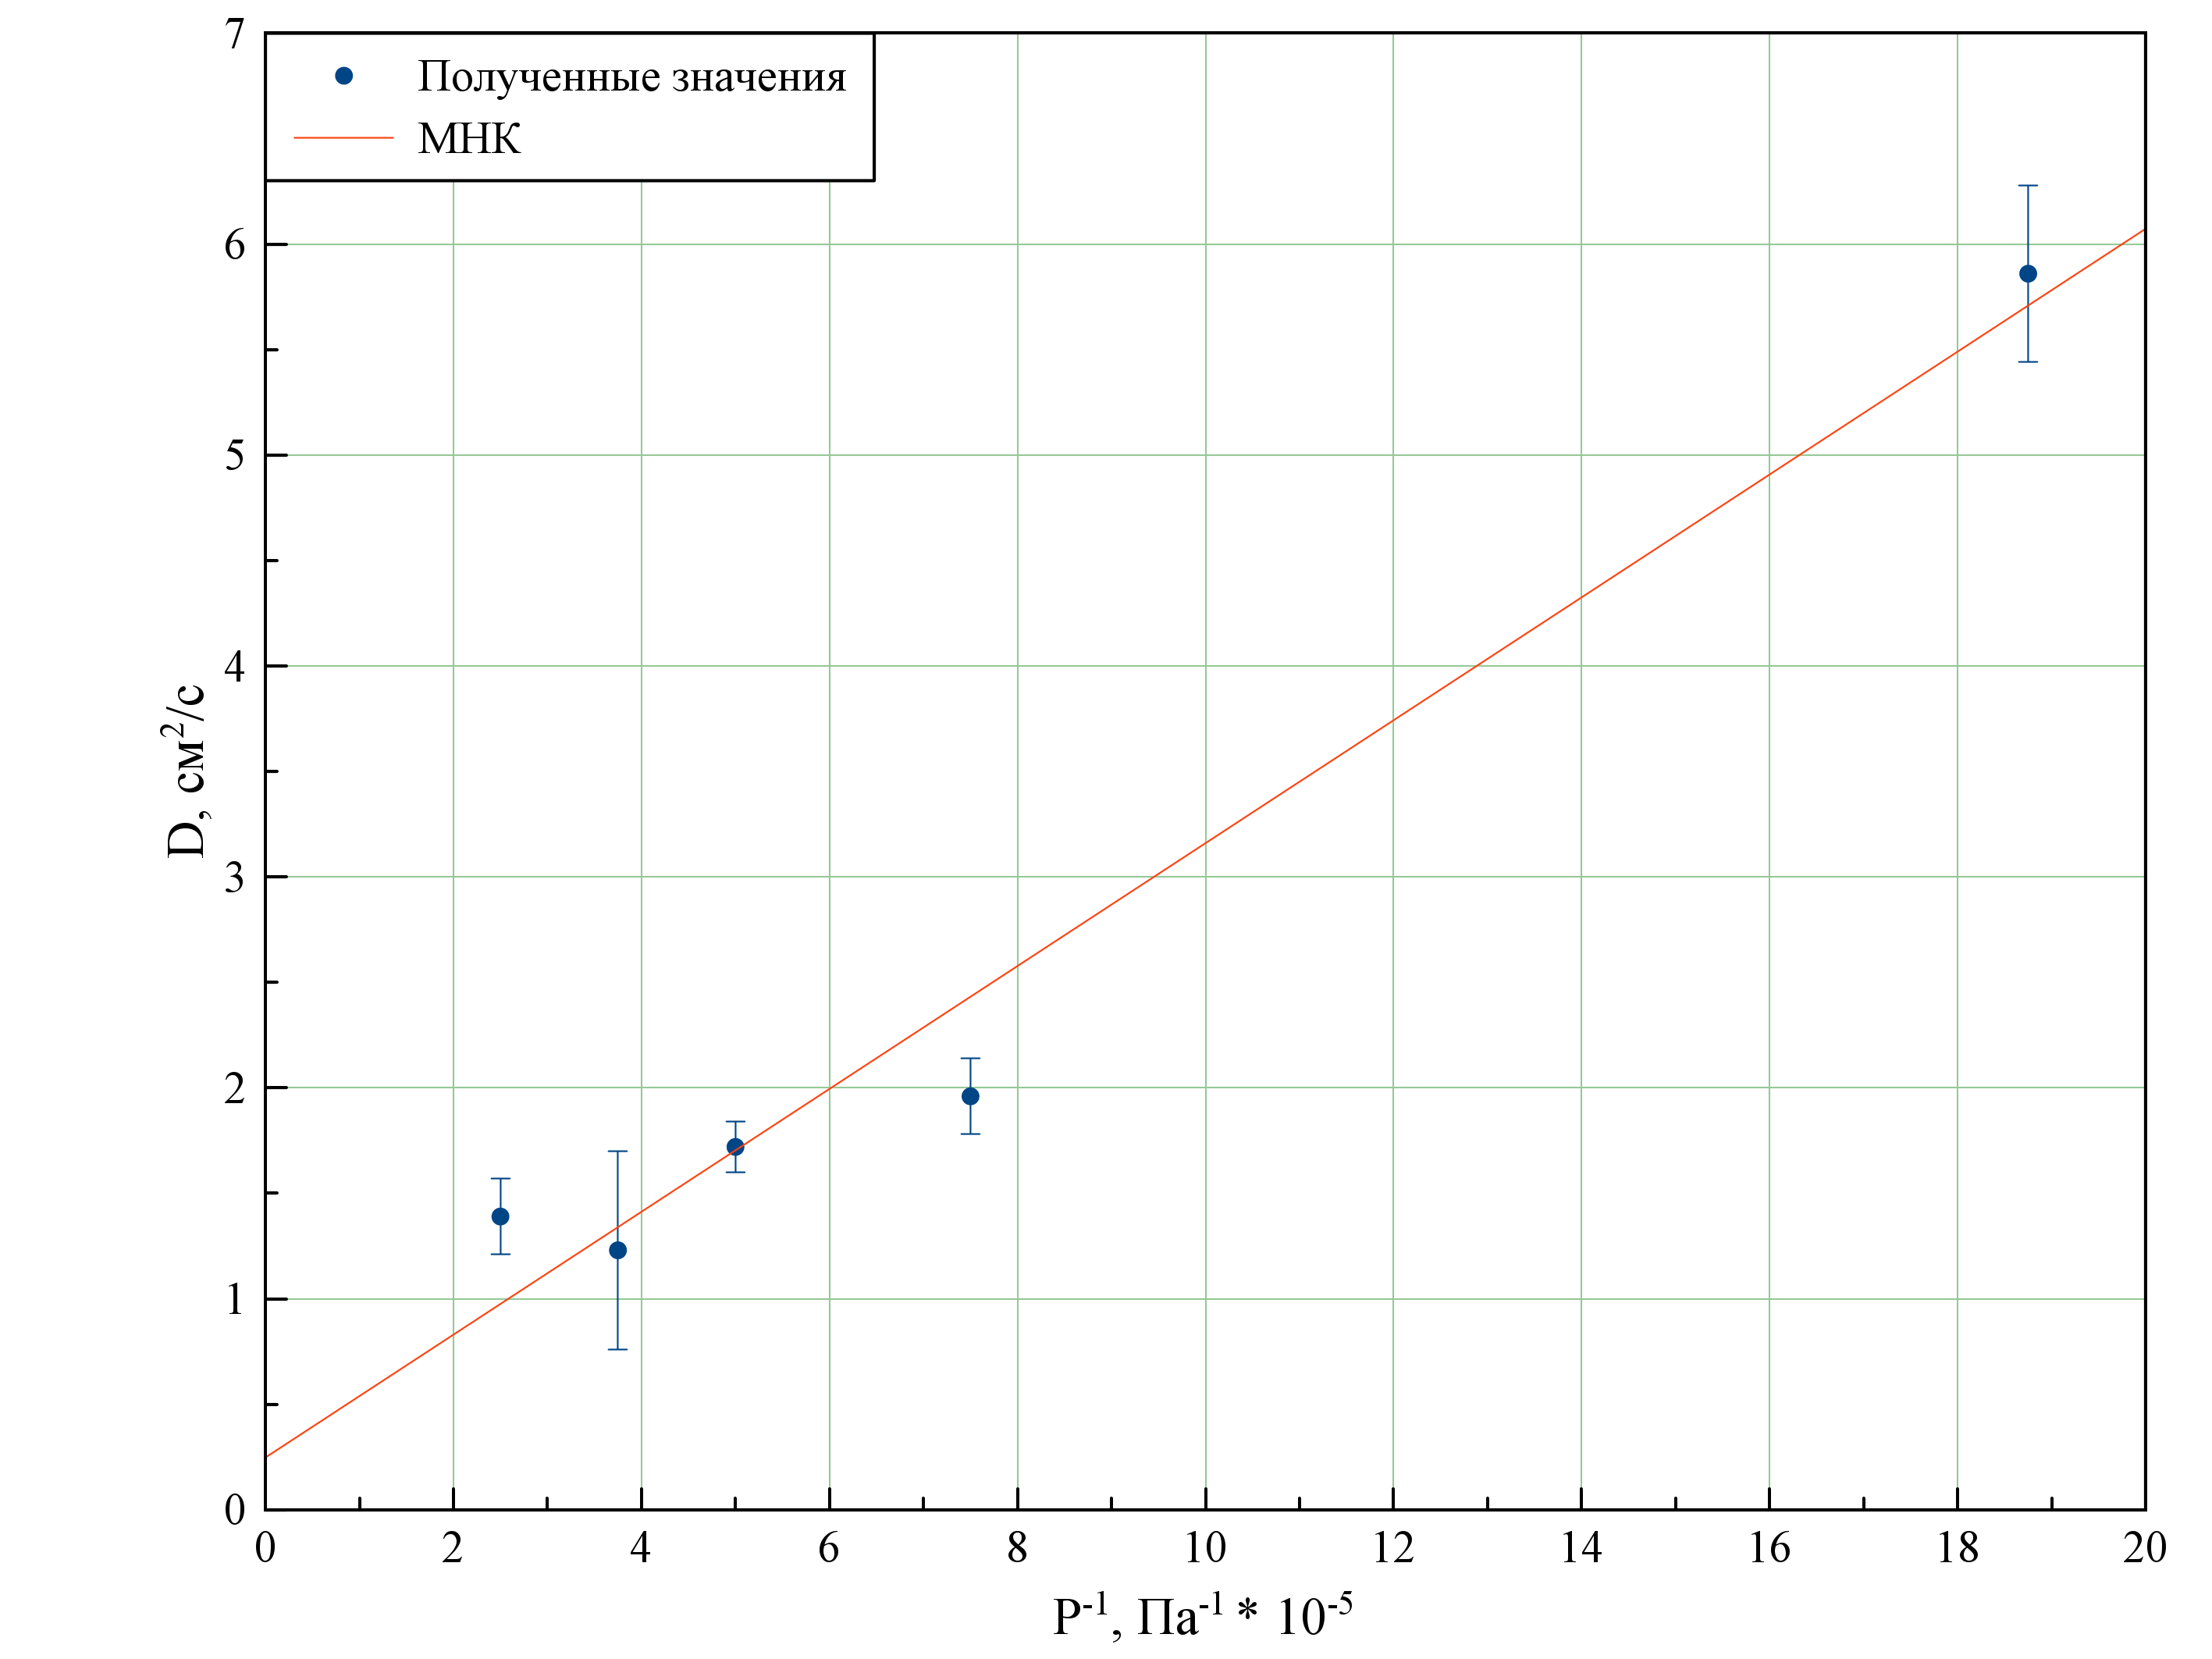
\includegraphics[width=1.0\textwidth]{graph6.png}
	\end{center}
\caption{график зависимости коэффициента диффузии от 1/P }
\end{figure}

2. Коэффициент диффузии при атмосферном давлении равен: $$ D = k \cdot \dfrac{1}{P_0}\text{, где }P_0 = 101 325 \text{ Па} $$
$$D = 18 799.9 \cdot \dfrac{1}{101325} = 0.186 \text{ } \dfrac{\textup{см}^2}{\textup{с}} $$
$$\sigma_D = \sigma_k \cdot \dfrac{1}{101325} = 875.1 \cdot \dfrac{1}{101325} =0.008 \text{ } \dfrac{\textup{см}^2}{\textup{с}} $$
\Large
В итоге получим: $ D = 0.186 \pm 0.008 \text{ } \dfrac{\textup{см}^2}{\textup{с}} $
\normalsize

\subsection{Длина свободного пробега}

$$D = \dfrac{1}{3}\cdot\lambda\cdot\stackrel{-}{v} = \dfrac{1}{3}\cdot\lambda\cdot\sqrt{\dfrac{8\cdot k\cdot N_{A}\cdot T}{\pi\cdot\mu}} 
\text{, где $\mu $ - приведенная масса смеси.} $$
$$\lambda = D \cdot 3 \cdot \sqrt{\dfrac{\pi\cdot\mu}{8\cdot k\cdot N_{A}\cdot T}} = 0.186 \cdot 10^{-4} \cdot 3 \cdot \sqrt{\dfrac{\pi\cdot 10^{-3}\cdot\dfrac{4\cdot 29}{4+29}}{8\cdot R\cdot 273}}= 4.35\cdot 10^{-8} \text{ м}$$

$$\sigma_{\lambda} = \sigma_{D} \cdot 3 \cdot \sqrt{\dfrac{\pi\cdot\mu}{8\cdot k\cdot N_{A}\cdot T}} = 0.02 \cdot 10^{-4} \cdot 3 \cdot \sqrt{\dfrac{\pi\cdot 10^{-3}\cdot\dfrac{4\cdot 29}{4+29}}{8\cdot R\cdot 273}}=  2\cdot10^{-9} \text{ м}$$

\Large
В итоге получим: $\lambda = 4.35 \pm 0.2 \cdot 10^{-8} \text{м}$
\normalsize

\subsection{Эффективное сечение столкновений атомов гелия с частицами воздуха}

$$\lambda = \dfrac{k\cdot T}{P_{0}\cdot\sigma} \text{; } $$
$$\sigma = \dfrac{k\cdot T}{P_0\cdot\lambda}=\dfrac{k\cdot 273}{101325\cdot 4.35\cdot 10^{-8}} =8.55 \cdot 10^{-19} \textup{ м}^2$$

\section{Сравнение полученных данных с теоретическими}

\noindent 1. Мы убедились что процесс диффузии подчиняется закону $\Delta n = \Delta n_{0}\cdot e^{\nicefrac{-t}{\tau}}$, так как графики в экспериментах представляют прямую в значениях погрешности;\\
2. Значение коэффициента диффузии 0.19 близко к табличному 0.62;\\
3. Полученные $\lambda$  и $\sigma$ порядково близки к аналогичным теоретическим значениям.

\end{document}